\documentclass[oneside]{book}
\usepackage{latexsym}
\usepackage{amsmath, amsthm, amssymb}
\usepackage{url}
\usepackage{graphicx}

\usepackage[spanish]{babel}
\usepackage[utf8]{inputenc}
\newtheorem{defi}{\bf Definici\'on}
%% \newtheorem{prop}{{\bf Proposici\'on}}[chapter]
%% \newtheorem{ob}{{\bf Observaci\'on}}[chapter]
%% \newtheorem{con}{{\bf Convenci\'on}}[chapter]
%% \newtheorem{teo}{{\bf Teorema}}[chapter]
%% \newtheorem{lema}{{\bf Lema}}[chapter]
\newtheorem{ejem}{\bf Ejemplo}
%% \newtheorem{dem}{{\bf Demostración}}
%% \newcommand{\inl}{\mathop{\sf inl}}
%% \newcommand{\inr}{\mathop{\sf inr}}
%% \newcommand{\abort}{\mathop{\sf abort}}
%% \newcommand{\void}{\mathop{\sf void}}

\title {Visualizaci\'{o}n del mercado de acciones en 3D}
\author{Juan Esteban Pemberthy\\\\ Juan Sebastian Munoz}
\date{\today}
\setcounter{tocdepth}{2}

\begin{document} 

\frontmatter

\maketitle
\tableofcontents
\chapter{Glosario}
\begin{enumerate}
	
\item \textbf{TDD (Test-driven development):} Desarrollo guiado por pruebas, es una práctica de programación que involucra otras dos prácticas: Escribir las pruebas primero (\textbf{Test First Development}) y Refactorización (\textbf{Refactoring}). Para escribir las pruebas generalmente se utilizan las pruebas unitarias (\textbf{unit test} en inglés). Primeramente se escribe una prueba y se verifica que las pruebas fallen, luego se implementa el código que haga que la prueba pase satisfactoriamente y seguidamente se refactoriza el código escrito. El propósito del desarrollo guiado por pruebas es lograr un código limpio que funcione (Del inglés: \textbf{Clean code that works}). La idea es que los requerimientos sean traducidos a pruebas, de este modo, cuando las pruebas pasen se garantizará que los requerimientos se hayan implementado correctamente.
\item \textbf{Pair Programming:} Programación en pareja,  requiere que dos Ingenieros en Software participen en un esfuerzo combinado de desarrollo en un sitio de trabajo. Cada miembro realiza una acción que el otro no está haciendo actualmente: Mientras que uno codifica las pruebas de unidades el otro piensa en la clase que satisfará la prueba, por ejemplo.
La persona que está haciendo la codificación se le da el nombre de controlador mientras que a la persona que está dirigiendo se le llama el navegador. Se sugiere a menudo para que a los dos socios cambien de papeles por lo menos cada media hora o después de que se haga una prueba de unidad.
\item \textbf{Mock Object:} Objeto simulado, los objetos simulados imitan el comportamiento de los objetos reales en forma controlada. Un programador generalmente escribirá un objeto simulado para probar el comportamiento de otro objeto en una forma muy similar a la que aplica un diseñador de carros al usar un muñeco para probar el comportamiento de un carro durante un accidente.
\item \textbf{RSpec:} Ruby Spec, es un framework para realizar tests en el lenguaje de programación Ruby, contiene su propio \textbf{framework} para simular objetos.
\item \textbf{ORM:} mapeo objeto-relacional, es una técnica de programación para convertir datos entre el sistema de tipos utilizado en un lenguaje de programación orientado a objetos y el utilizado en una base de datos relacional. En la práctica esto crea una base de datos orientada a objetos virtual, sobre la base de datos relacional. Esto posibilita el uso de las características propias de la orientación a objetos (básicamente herencia y polimorfismo).
\item \textbf{MVC:} Modelo Vista Controlador, es un patrón de arquitectura de software que separa los datos de una aplicación, la interfaz de usuario, y la lógica de control en tres componentes distintos. El patrón MVC se ve frecuentemente en aplicaciones web, donde la vista es la página HTML y el código que provee de datos dinámicos a la página. El modelo es el Sistema de Gestión de Base de Datos y la Lógica de negocio, y el controlador es el responsable de recibir los eventos de entrada desde la vista.
\item \textbf{Daemon:} Un demonio, (siglas en inglés, \textbf{Disk And Execution Monitor}), es un tipo especial de proceso informático que se ejecuta en segundo plano en vez de ser controlado directamente por el usuario. Este tipo de programas se ejecutan de forma continua (infinita), vale decir, que aunque se intente cerrar o matar el proceso, este continuará en ejecución o se reiniciará automáticamente. Todo esto sin intervención de terceros y sin dependencia de consola alguna.
\item \textbf{Unity3D:} Motor de Juegos para crear aplicaciones 3D.
\item \textbf{Shader:} Conjunto de instrucciones gráficas destinadas para el acelerador gráfico, estas instrucciones dan el aspecto final de un objeto. Los Shaders determinan materiales, efectos, color, luz, sombra y etc.
\item \textbf{Vertex Shaders:} Actúa sobre las coordenadas, color, textura, etc. de un vértice.
\item \textbf{Geometry Shaders:} Es capaz de generar nuevas primitivas dinamicamente.
\item \textbf{Pixel Shaders:} Actúa sobre el color de cada pixel (texel para ser más preciso).
\item \textbf{Mesh:} Término que se refiere a una figura en 3D, en general que esté formada por polígonos.
\item \textbf{Triangulación de Delaunay:} Es una red de triángulos que cumple la condición de Delaunay. Esta condición dice que la circunferencia circunscrita de cada triángulo de la red no debe contener ningún vertice de otro triángulo. Se usan triangulaciones de Delaunay en geometría por ordenar, especialmente en gráficos 3D por computadora.
\item \textbf{Transform:} Objeto en Unity3D que describe propiedades de un \textbf{Mesh} como Escalamiento, Rotación, Posición, etc.
\item \textbf{Proyección Ortográfica:} Esta proyección utliza rayos paralelos para crear una imágen de la escena. El área de vision está determinada por las longitudes de los vectores \textbf{right} y \textbf{up}, que, por cierto, han de ser especificados, ya que con este tipo de proyección no se utilizan los de la cámara por defecto. En caso de ser omitidos, se usará el segundo método de proyección ortográfico de la cámara.
\item \textbf{Proyección Perspectiva:} La palabra clave \textbf{perspective} determina la cámara perspectiva, que simula la típica cámara con objetivo. El ángulo de visión horizontal es determinado por la proporción entre la longitud del vector dirección y la longitud del vector \textbf{right}, o por la palabra clave opcional \textbf{angle}, que es el modo aconsejado. El ángulo de visión ha de ser mayor de 0 y menor de 180 grados.
\item \textbf{Framework:} En el desarrollo de software, es una estructura de soporte definida, mediante la cual otro proyecto de software puede ser organizado y desarrollado. Típicamente, puede incluir soporte de programas, bibliotecas y un lenguaje interpretado entre otros software para ayudar a desarrollar y unir los diferentes componentes de un proyecto.
Representa una arquitectura de software que modela las relaciones generales de las entidades del dominio. Provee una estructura y una metodología de trabajo la cual extiende o utiliza las aplicaciones del dominio.
\item \textbf{Agile Software Development:} Desarrollo ágil de software, se entiende como Desarrollo ágil de software a un paradigma de Desarrollo de Software basado en procesos ágiles. Los procesos ágiles de desarrollo de software, conocidos anteriormente como metodologías livianas, intentan evitar los tortuosos y burocráticos caminos de las metodologías tradicionales enfocándose en la gente y los resultados.
Es un marco de trabajo conceptual de la ingeniería de software que promueve iteraciones en el desarrollo a lo largo de todo el ciclo de vida del proyecto. Existen muchos métodos de desarrollo ágil; la mayoría minimiza riesgos desarrollando software en cortos lapsos de tiempo. El software desarrollado en una unidad de tiempo es llamado una iteración, la cual debe durar de una a cuatro semanas. Cada iteración del ciclo de vida incluye: planificación, análisis de requerimientos, diseño, codificación, revisión y documentación. Una iteración no debe agregar demasiada funcionalidad para justificar el lanzamiento del producto al mercado, pero la meta es tener un demo (sin errores) al final de cada iteración. Al final de cada iteración el equipo vuelve a evaluar las prioridades del proyecto.
\item \textbf{CoC:} Convención sobre Configuración, es un paradigma de programación de software que busca decrementar el número de decisiones que un desarrollador necesita hacer, ganando así en simplicidad pero no perdiendo flexibilidad por ello.
Cuando la convención tomada es suficiente para lograr el comportamiento deseado, se hace innecesario realizar aquellas tareas para las que la convención ya ha definido un comportamiento, por ejemplo escribir archivos XML de configuración del entorno. Cuando la convención definida no es suficiente para lograr el comportamiento deseado, el desarrollador puede alterar el comportamiento por defecto y adaptarlo a sus necesidades.
\item \textbf{Don't Repeat yourself (DRY):} El principio No te repitas, es una filosofía de definición de procesos que promueve la reducción de la duplicación especialmente en computación. Según este principio ninguna pieza de información debería estar duplicada nunca debido a que la duplicación incrementa la dificultad en los cambios y evolución posterior, puede perjudicar la claridad y crea un espacio para posibles inconsistencias. Por `pieza de información' podemos, en un sentido amplio, entender desde datos almacenados en una base de datos pasando por el código fuente de un programa de software hasta llegar a información textual o documentación.
Cuando el principio DRY se aplica de forma eficiente los cambios en cualquier parte del proceso requieren cambios en un único lugar. Por el contrario, si algunas partes del proceso están repetidas por varios sitios, los cambios pueden provocar fallos con mayor facilidad si todos los sitios en los que aparece no se encuentran sincronizados.
\end{enumerate}
\chapter{Introducción}

\begin{quote} \textit{``A good Notation has a sublety and suggestiveness which at
  times makes it almost seem like a live teacher.''}
  \\ --Bertrand Russell\footnote{Prólogo del capítulo \textit{``Minilanguages: Finding a
    Notation that Sings''} en \textit{``The art of Unix Programming''} por Eric Raymond.}
\end{quote} 

La idea de permitir al usuario crear y modificar operadores dentro del lenguaje de
programación tiene como objetivo permitir sintaxis más concisa. Algunos lenguajes de
programación permiten al programador definir sus propios operadores
infijos(~\cite{jones:haskell},~\cite{leroy:ocaml}). Otros permiten el concepto más
general de operador disfijo(~\cite{Coq},~\cite{goguen:obj},~\cite{clavel:maude} y
otros). Operadores disfijos son descritos en~\cite{jones:distfix} y
~\cite{Aasa:UDS}. Escencialmente se trata de operadores de una o mas partes que
pueden traer los argumentos embebidos en si mismos. Un ejemplo tomado de OBJ es el 
siguiente:

\begin{verbatim}
op if_then_else_fi : Bool Int Int -> Int .
\end{verbatim}

La idea de este trabajo se centra en el estudio de los operadores permisivos 
como mecanismo de extensibilidad en un lenguaje de programación. 

El capitulo 1 es un breve recuento de los objetivos generales y específicos. El
capítulo 2 hace un recorrido sobre diferentes conceptos necesarios para este
trabajo. El capítulo 3 justifíca este trabajo en el área de diseño de lenguajes de
programación. El capítulo 4 explica los detalles de diseño y diferentes estrategias
utilizadas para el \textit{``parsing''} y evaluación de operadores distfijos
permisivos. El capítulo 5 ilustra como puede utilizarse el lenguaje de programación
como mecanísmo de extensibilidad para construir características
pseudo-objetuales. Finalmente el capitulo 6 describe las conclusiones respecto la
implementación de dicho lenguaje y describe posible trabajo futuro alrededor de la
inclusión de operadores permisivos.












  


%%% Local Variables: 
%%% mode: latex
%%% TeX-master: "tesis"
%%% End: 

\chapter{Objetivos}
\section{Objetivo General}
Exploración del uso de operadores disfijos permisivos en un lenguaje fuertemente tipado.
\section{Objetivos Específicos}
\begin{itemize}
\item Entender que son los operadores disfijos.
\item Implementar un lenguaje de programación prueba de concepto que simule operadores
  disfijos mediante el lenguaje de programación Haskell.
\item Utilizar los operadores disfijos del lenguaje como mecanismo de
  extensibilidad para implementar un lenguaje con características
  objetuales. Dicha construcción se realizará en etapas.
\end{itemize}


\mainmatter
\chapter{Objetivos del proyecto}
\section{Objetivo General}
Brindar un mecanismo que permita visualizar y comparar el movimiento de una o varias acciones de la bolsa de valores de Colombia en el tiempo, mediante contenidos en tercera dimensión, incursionando en un campo sobre el cuál la mayoría de aplicaciones están diseñadas para desplegar sus resultados en 2D.
\section{Objetivos Específicos}
\begin{itemize}
\item Permitir llevar el control e historial de acciones de manera personalizada.
\item Desarrollar un protocolo de comunicación que pueda ser reutilizado en aplicaciones futuras, que exploten el poder del motor gráfico para desarrollar contenidos alimentados desde una base de datos.
\item Integrar el modelo de datos con la aplicación 3D para desplegar apropiadamente el movimiento del mercado y/o una determinada acción. 
\end{itemize}
\chapter{Alcance y productos esperados}
Se entrega una aplicación Web desarrollada en \textbf{Ruby on Rails} que integra un conjunto de contenidos en 3D desarrollados en \textbf{Unity 3D} un motor gráfico que permite exportar los contenidos para que sean acoplados con la aplicación Web y consecuentemente se puedan visualizar desde un navegador. Además los contenidos se estarán actualizando constantemente en un período de tiempo razonable, a esto se le suma la posibilidad de un usuario registrarse y configurar su perfil, sobre este perfil cada usuario podrá simular o evidenciar según sea el caso ( sí posee ó no acciones en la vida real) ganancias o pérdidas sobre las acciones que tenga registradas y la cantidad asociada a las mismas.\\

Se  aclara de antemano que la aplicación no sirve como medio para comprar o vender acciones, en el perfil también se puede desplegar de forma personalizada el movimiento de las acciones que el usuario tenga registradas, permitiendo diferentes esquemas de visualización en los que por ejemplo se tendrá en cuenta información guardada en la base de datos de la aplicación, por ejemplo los periodos de tiempo en los que un usuario registró una compra o venta serán utilizados para ayudar  al usuario a que se de una mejor idea del estado de su inversión.\\

Adicionalmente los clásicos esquemas en segunda dimensión que actualmente son utilizados para la representación del movimiento de acciones como lo son las barras, también fueron implementados en la aplicación, pero de tal manera que tales barras no muestren sólo el estado de una acción en varios periodos de tiempo, o varias acciones en un periodo de tiempo, sino ofrecer la oportunidad de ver varias acciones como se comportan en varios periodos de tiempo.
\chapter{Justificación}
El uso de tecnologías de visualización, como apoyo al entendimiento de datos planos en diferentes entornos, tanto de ingeniería como administrativos es un tema que día a día ha venido tomando auge en nuestra sociedad, debido a que facilitan la comprensión de como se están comportando dichos datos para consecuentemente ayudar en un momento determinado con la toma de decisiones.\\

Al facilitar una herramienta que permita visualizar los datos del mercado de acciones, no solo en el tiempo para una sola acción, sino también entre diferentes acciones a la vez, se abre la posibilidad de comparar rendimientos o pérdidas de una o varias acciones a través del tiempo, dentro de un mismo gráfico, para así mirar tendencias y tomar decisiones.\\

El planteamiento de la solución acá expuesta se basa en la necesidad de tener mas control y conocimiento sobre un portafolio que una persona determinada maneje, independientemente de donde esta se encuentre, pues gracias a la ayuda de la tecnología y mas específicamente de la Web 2.0, acceder desde cualquier computador a un mismo portafolio es completamente transparente para quien lo usa. De esta forma, los usuarios podrán tener acceso a su portafolio de acciones en tiempo real, en el que encuentran tablas y gráficos que representan el historial de sus inversiones. 

\chapter{Conclusiones}



\chapter{Solución}

Teniendo clara una necesidad y/o problema a suplir/solucionar, se analizaron varias tecnologías y patrones de desarrollo que permitirían llevar a cabo el desarrollo de una aplicación web, en la que fuera posible visualizar contenidos en 3D que fueran alimentados por una Base de Datos.\\

Las herramientas seleccionadas fueron, \textbf{Ruby on Rails}\footnote{http://rubyonrails.org/} para desarrollar la aplicación web, pensando en un metodología ágil de desarrollo, y que a su vez permitiera que los contenidos fueran fáciles de integrar, el motor de bases de datos elegido fue \textbf{MySql}, por otro lado, se elegió \textbf{Unity3D}\footnote{http://unity3d.com/} por su capacidad de generar contenidos 3D que se apoyan directamente de las tarjetas aceleradoras de video para visualizar dichas escenas, además cuenta con una API que facilita exportar contenidos para que sean visibles en un navegador.\\

\section{¿Por qué Ruby on Rails?}

Para responder a esta pregunta, es necesario primero definir a \textbf{Ruby on Rails}, llamado tambien \emph{Rails} ó RoR, es un \emph{framework} que hace que sea más fácil desarrollar, implementar, y mantener aplicaciones web. Durante los meses que siguieron a su primera liberación, \emph{Rails} paso de ser un juguete desconocido a un fenomeno mundial. Ha ganado premios, y más importante aún, se ha convertido en el framework de preferencia para la implementación de cierto conjunto de las llamadas aplicaciones Web 2.0\cite{ror:awdwr}.\\

Se eligió \emph{Rails} para desarrollar la aplicación web en la que se comunican datos y contenidos 3D, por qué se buscaba utilizar una herramienta en la que la convención estuviera por encima de la configuración\footnote{Léase \textbf{CoC} en el glosario}, que contará con una arquitectura pre definida, en éste caso MVC (Modelo Vista Controlador) Figura\ref{fig:mvc} que \emph{Rails} aprovecha apropiadamente, cuándo se desarrolla en \emph{Rails}, hay un lugar para cada pieza de código\footnote{Léase \textbf{DRY} en el glosario}, y todos los componentes de la aplicación interactúan según el estándar.\\

\begin{figure}[h]
	\centering
		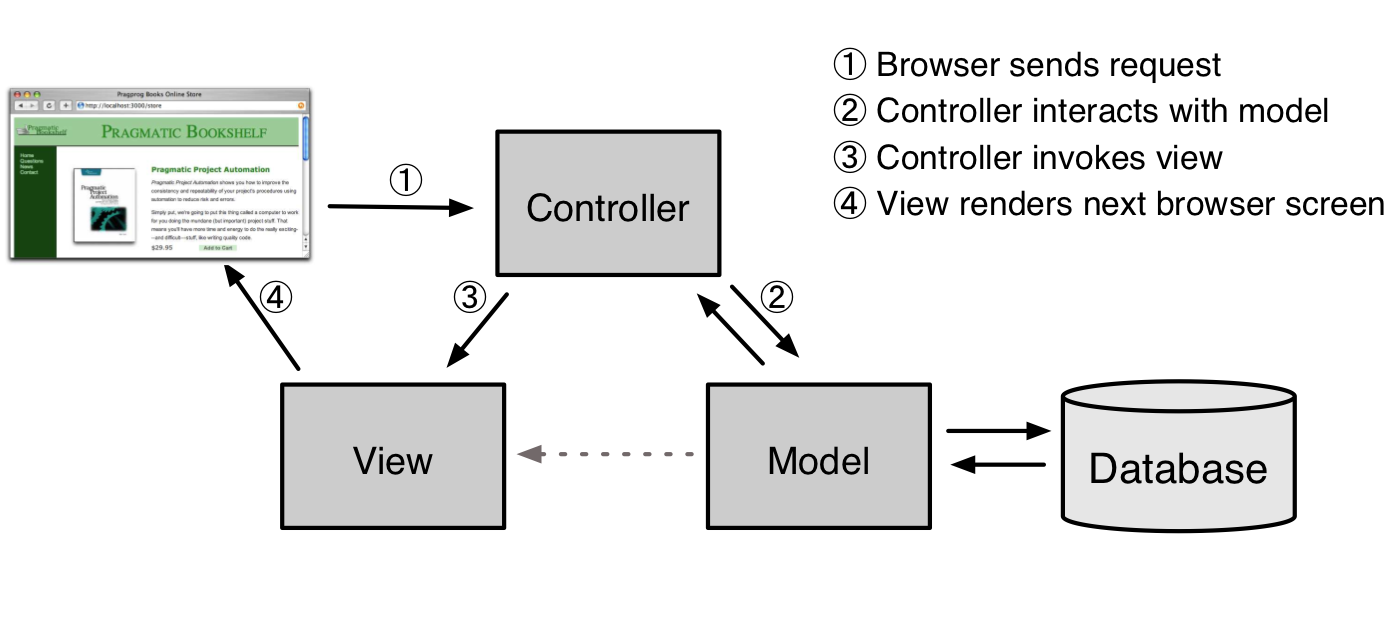
\includegraphics[scale=0.25]{mvc.PNG}
		\caption{Modelo Vista Controlador}
	\label{fig:mvc}
\end{figure}

Los programadores profesionales, suelen escribir tests para simular el comportamiento de la aplicación que se esta desarrollando, para el presente proyecto, se buscaba que el framework tuvieran un soporte para hacer tests, una vez más Rails se ajusta a esas necesidades, pues cuenta con soporte para algunos frameworks para realizar tests, se encuentran; RSpec (utilizada en este proyecto, bajo la filosofía de TDD \footnote{Léase \textbf{TDD} en el glosario}) en donde se escriben los tests, antes de la implementación, Test Unit, Shoulda y Cucumber (BDD\footnote{Léase \textbf{BDD} en el glosario})\\

Se buscaba que la herramienta fuera escrita en un lenguaje de programación orientado a objetos e interpretado, por la necesidad de crear \emph{scripts} que corrieran independiente de la aplicación, como tareas programadas para correr cada cierto tiempo. Las aplicaciones en \emph{Rails} son escritas en el lenguaje de programación \emph{Ruby}, que cumple con lo que se buscaba, y aparte introduce características favorables como metaprogramación, haciendo que el código sea más fácil de entender, leer y/o escribir, programas más cortos en términos de \textbf{LOC}\footnote{Líneas de código, en inglés \emph{Lines of Code}}, para evidenciar esto, a continuación se muestra una porción de código de la aplicación, en la que se define una clase de un Modelo que expresa mucha información en pocas líneas de código y es fácil de entender. \newpage

\begin{verbatim}
class Record < ActiveRecord::Base  

  belongs_to :stock_action

  validates_presence_of :amount
  validates_presence_of :price
  validates_presence_of :variation

  validates_numericality_of :price, :amount, :greater_than => 0
  validates_numericality_of :variation

end
\end{verbatim}

Finalmente, no se pretendía manipular la base de datos directamente, es decir, con código nativo del motor de bases de datos, sino sacar provecho de técnicas como ORM \footnote{Léase \textbf{ORM} en el glosario}, en las que las tablas de las bases de datos son mapeadas a clases, los registros de las tablas son mapeados como objetos, y consecuentemente los campos, se mapean como atributos de los objetos, mientras que existen metodos de clases que se encargan de realizar operaciones a nivel de tablas, dejando como opcional la utilización de código \textbf{SQL} dentro de la aplicación, una vez más \emph{Rails} suple esta necesidad con \textbf{ActiveRecord} ó \textbf{Datamapper}.

\section{¿Por qué Unity3D?}

Actualmente existen posibilidades para el desarrollo de interfaces gráficas de usuario tridimensionales en los navegadores de internet, \textbf{PaperVision3D}\footnote{\textbf{Papervision} es un motor de gráficos para Flash. Aunque todavía está en versión beta, ya se han lanzado algunas aplicaciones que lo utilizan y los resultados son muy prometedores.} (entre otros) es un motor de renderizado 3D en tiempo real, escrito en \textbf{ActionScript 3}\footnote{\textbf{ActionScript} es un lenguaje de programación orientado a objetos (OOP), utilizado en especial en aplicaciones web animadas realizadas en el entorno \textbf{Adobe Flash}}, de código abierto entre otros, que posee las funcionalidades básicas de la computación gráfica tridimensional, creando una ilusión 3D en el motor de renderizado que posee el \emph{Flash Player}. \\

Desafortunadamente el motor de renderizado para \emph{Flash} esta diseñado específicamente para gráficos en 2D. Este es un punto crítico por el cual \emph{Flash} no es técnicamente la mejor opción. La cantidad de fotogramas de contenido 3D renderizados por segundo (FPS)\footnote{Las imágenes por segundo (en inglés más conocido como \emph{frames per second, fps}) es la medida de la frecuencia a la cual un reproductor de imágenes genera distintos fotogramas (\emph{frames}). En informática estos fotogramas están constituídos por un número determinado de pixeles que se distribuyen a lo largo de una red de texturas para determinar un fotograma por segundo.\\
La frecuencia es proporcional al número de pixeles que se deben generar, incidiendo en el rendimiento de la máquina.} suele ser media o baja, en casos reales. La comunidad de desarrolladores del \emph{Flash Player} está desarrollando varios proyectos para poder renderizar 3D en el mismo, existen proyectos privados y de código abierto, entre los que se encuentran: \\
\begin{itemize}
\item[$\bullet$] \emph{Alternativa3D} 
\item[$\bullet$] \emph{Away 3D} 
\item[$\bullet$] \emph{Five3D} 
\item[$\bullet$] \emph{ND3D} 
\item[$\bullet$] \emph{Papervision3D} 
\item[$\bullet$] \emph{Sandy3D} 
\item[$\bullet$] \emph{Wire Engine 3D}
\end{itemize} 
Los cuales usualmente utilizan algoritmos de rasterizado para el proceso de generar una imagen 2D a partir de una escena 3D, consumiendo así en dicho proceso, mucha capacidad computacional.\\

La técnica más utilizada hoy en día para la producción de gráficos 3D en tiempo real es la rasterización. La rasterización es básicamente un proceso de transformación de datos de vectores que se convierten en un conjunto de pixeles (imágenes).\\

En pocas palabras, muchos de los motores de renderizado 3D escritos para trabajar con el \emph{plugin} de \emph{Flash}  utilizan bastante lógica para producir una ilusión 3D sobre 2D debido a que es una de las técnicas mas rápidas, pero, como se mencionó anteriormente, estos motores por mas optimizados que estén, siempre van a depender del renderizado 2D para el cual fue diseñado \emph{Flash} en un principio.\\

\textbf{Unity3D} por su parte también es un \emph{plugin} para navegadores, especializado en la creación de contenido 3D en tiempo real. Técnicamente es la mejor opción para desarrollo 3D, pues dicho \emph{plugin} aprovecha las capacidades de procesamiento de hardware de la tarjeta de video para desplegar contenidos en 3D, permitiendo así optimizar ciclos de procesamiento en el mejoramiento de los FPS de la escena en vez de ejecutar cálculos de conversión de imágenes 3D a 2D, repercutiendo enormemente en la experiencia del usuario.\\

\emph{Unity3D} por su parte es un motor escrito en C/C++ que trabaja con \emph{Mono}\footnote{\textbf{Mono} es el nombre de un proyecto de código abierto iniciado por Ximian y actualmente impulsado por Novell (tras la adquisición de Ximian) para crear un grupo de herramientas libres, basadas en GNU/Linux y compatibles con .NET según lo especificado por el ECMA.} y \emph{PhysX}\footnote{\textbf{PhysX} es un chip y un kit de desarrollo diseñados para llevar a cabo cálculos físicos muy complejos. Conocido anteriormente como la SDK de NovodeX, fue originalmente diseñada por AGEIA y tras la adquisición de AGEIA, es actualmente desarrollado por Nvidia e integrado en sus chip gráficos más recientes.} para crear código multiplataforma, haciendo así practicamente transparente generar ejecutables tanto para MacOSX, Windows, widgets y exportar para Web.\\

Gracias a Mono, es fácil generar ejecutables multiplataforma debido a la arquitectura con la que dicho \emph{framework} trabaja. Figura\ref{fig:mono}\\

\begin{figure}[h]
	\centering
		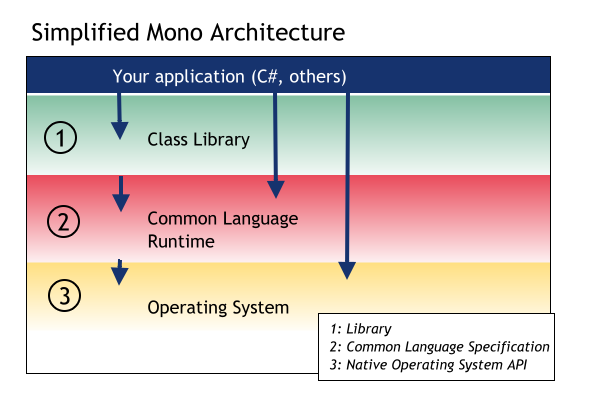
\includegraphics[scale=0.6]{Mono.PNG}
		\caption{Arquitectura general del \emph{framework} Mono}
	\label{fig:mono}
\end{figure}


Por otro lado, \emph{Unity3D} también se aprovecha de la capacidad del motor de física \emph{PhysX} para llevar a cabo cálculos complejos para así alivianar la carga de procesamiento que conlleva un juego/aplicación 3D.\\

Cuando el Motor exporta contenido a Web, dicho contenido se puede comunicar facilmente con \emph{Javascript}, permitiendo así entablar un puente de comunicaciones con \emph{Rails} a través de \emph{Javascript}, factor clave para la visualización de los datos que tiene la aplicación.\\

\section{¿Cómo se complementan estas dos tecnologías?}

Como se justificó en las secciones anteriores, tanto \emph{Rails} como \emph{Unity3D} son herramientas sobre las que se puede desarrollar efectivamente tanto aplicaciones Web convencionales, así como aplicaciones 3D, pero era necesario que ambas tuvieran la forma de recibir y enviar mensajes a través de un protocolo de comunicación, de tal manera que fuera transparente una llamada de una aplicación a la otra como si se tratase de una llamada local.\\

Dicho protocolo de comunicación, fue soportado por \textbf{Javascript} puesto que \emph{Rails} cuenta con una librería bien soportada para convertir datos nativos de \emph{Ruby} a \emph{Javascript} y ya que el contenido generado por \emph{Unity3D} tiene una API accequible escrita en \emph{Javascript} para controlar el estado del contenido dentro del browser, haciendo entonces a \emph{Javascript} la herramienta óptima para comunicar ambas tecnologias.\\


\chapter{Desarrollo de la aplicación.}

\section{Desarrollo Web.}

A continuación se describe detalladamente el proceso de construcción que se utilizó para el desarrollo de la aplicación web, seguiendo el estándar de \emph{Rails}, se adoptó una metodología ágil\footnote{Es un proceso de desarrollo de software, desarrollado inicialmente por James Martin en 1980. El método comprende el desarrollo iterativo, y la construcción de prototipos, tiende a englobar también la usabilidad, utilidad y la rapidez de ejecución.} buscando velocidad en el desarrollo del producto, así como calidad, pues la aplicación supliría las necesidades de los usuarios y se entregaría en un tiempo acorde según los límites de tiempo del proyecto.

\subsection{Especificaciones.}

El primer paso para desarrollar apropiadamente una aplicación guiada por tests(\emph{Test Driven Development - TDD}), es definir las especificaciones que determinan el comportamiento del sistema, dichas especificaciones más tarde se convertirán en la base de los tests para el desarrollo de la aplicación.\\

En este punto, se describió la aplicación Web a ser escrita teniendo en cuenta la definición del problema y el marco referencial, la tarea principal entonces sería integrar datos con contenidos para lograr el desarrollo final de la aplicación, después de tener claro la necesidad a cubrir y de que se necesitaba brindar un ambiente de fácil acceso y manipulación para los usuarios, se decidió desarrollar una aplicación web con las siguientes especificaciones(especificaciones que mas tarde se ampliarían para la construcción de los test.):


\begin{itemize}
\item[$\bullet$] Sistema de usuarios protegido por contraseña.
\item[$\bullet$] Cada usuario puede registrar un portafolio.
\item[$\bullet$] Cada portafolio esta compuesto por títulos.
\item[$\bullet$] Los títulos representan el estado personal de una acción registrada por el usuario, para de esa manera determinar, si la inversión le representa a su propietario una perdida o una ganancia.
\item[$\bullet$] Dentro del portafolio se pueden agregar, actualizar, comparar y eliminar títulos.
\item[$\bullet$] Cada título puede ser seleccionado para inspeccionar su comportamiento durante un rango de tiempo determinado por el usuario.
\item[$\bullet$] Los títulos de cada usuario pueden ser comparados simultáneamente con el apoyo de los contenidos 3D.
\item[$\bullet$] Los títulos se basan en la información que se obtiene al actualizar las acciones.
\item[$\bullet$] Las acciones se actualizan cada veinte minutos cuándo el mercado esta abierto.
\item[$\bullet$] La página principal no necesita registro, evidencia el comportamiento del mercado con una gráfica en 3D y muestra el estado actual de cada acción.
\end{itemize}

\subsection{Definición de modelos.}

Con el comportamiento de la aplicación claro, era necesario entonces definir los datos con los que la misma trabajaría, que tablas se necesitarían, que campos, y que tipos de datos estarían siendo manipulados por la aplicación, y cuáles  alimentarían los contenidos 3D.\\

Aparte de los definición de los modelos involucrados, se buscaba estar en la capacidad de trabajar bajo un patrón \textbf{ActiveRecord}\footnote{Es un enfoque al problema de acceder a los datos de una base de datos. Una fila en la tabla de la base de datos se envuelve en una clase, de manera que se asocian filas únicas de la base de datos con objetos del lenguaje de programación usado. Cuando se crea uno de estos objetos, se añade una fila a la tabla de la base de datos. Cuando se modifican los atributos del objeto, se actualiza la fila de la base de datos. La clase envoltorio implementa métodos de acceso para cada columna de la tabla o vista.} pensando en un enfoque \textbf{ORM}\footnote{Léase \textbf{ORM} en el glosario.} que permitiera manipular los registros de la base datos como si se trataran de objetos definidos en el lenguaje de programación \emph{Ruby}.\\

El modelo entidad relación final, y que representa la estructura de la base de datos de la aplicación es el que se muestra en la Figura \ref{fig:erd}, según la información recogida de las especificaciones, era claro que se necesitaba un modelo que representara los usuarios, a su vez dichos usuarios tienen relacionado un portafolio(relación \emph{1..1}), cada portafolio actúa como contenedor de títulos(relación \emph{1..n}), indirectamente entonces, el usuario posee títulos, como sucede en la vida real, el modelo \emph{stock\_action} representa la acción real en el mercado, y sobre la cual existen múltiples títulos asociados.

\begin{figure}[h]
	\centering
		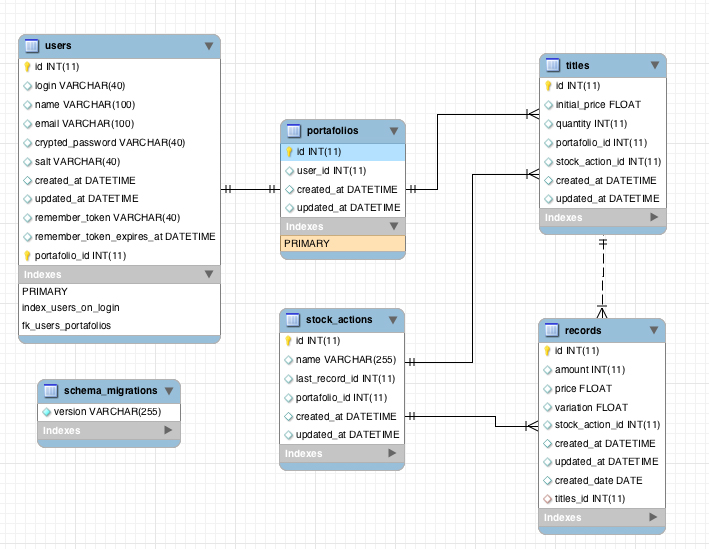
\includegraphics[scale=0.5]{erb_mertd.jpg}
		\caption{Modelo Entidad Relación - Mertd(Mercado 3D)}
	\label{fig:erd}
\end{figure}

Finalmente el modelo \emph{record} es sobre el cual se registran todos los movimientos de las acciones, es decir, sobre el que se hacen las actualizaciones según el estado de una acción, por ejemplo, cada vez que se obtiene información nueva indicando el estado de una acción, un registro nuevo es agregado y guardado en este modelo, luego este registro es usado por otros modelos para calcular el estado de una inversión de forma personalizada.\\

La siguiente porción de código de la aplicación, muestra claramente cómo se puede sacar provecho al utilizar un patrón como \textbf{ActiveRecord}, según este patrón, si existe una tabla \emph{titles} debe haber una clase \emph{Title} asociada, sobre la cual se hace el mapeo.

\begin{verbatim}
	t = Title.new
	t.initial_price = 15250.66
	t.quantity = 10000
	t.portafolio = p #p es un portafolio existente cuya id es 1
	t.stock_action = s_a #s_a es una acción existente cuya id es 15
	t.save
	#otra manera mas corta de hacer este regristro, podría ser:
	#t = Title.new(:initial_price => 15250.66, :quantity => 10000, 
	#			   :portafolio => p, :stock_action => s_a)
	#
\end{verbatim}

A nivel de bases de datos, las anteriores declaraciones son interpretadas de la siguiente manera:

\begin{verbatim}
INSERT INTO titles 
  (initial_price, quantity, portafolio_id, stock_action_id) 
  VALUES (15250.66, 10000, 1, 15);
\end{verbatim}

Cabe resaltar que siempre será más rápido ejecutar directamente el código nativo interpretado por el motor de base de datos, pero en éste caso se opto por la claridad de código y la manipulación de objetos pues no se requirió diseñar consultas que hicieran que la diferencia de tiempos entre uno y otro método fuera considerable.

\subsection{Configuración.}

Al tratarse de una aplicación web, la configuración estuvo enfocada en la determinación de que servidores web utilizar, y que motor de bases de datos, así como la integración de estos con la aplicación.

\subsubsection{Servidor Web - \emph{Clusters}}

En el lado de los servidores, se eligió \textbf{Mongrel}\footnote{Es una libreria HTTP y un servidor web para aplicaciones escritas en \emph{Ruby}. Una característica de \emph{Mongrel} es que usa HTTP plano, en vez de \emph{FastCGI} ó \emph{SCGI}, para comunicarse con otros servidores que podrían estar una capa encima de éste.}, encargado de correr la aplicación web a modo de \emph{clusters},\footnote{Los \emph{Mongrel Clusters} son un conjunto de procesos de \emph{Mongrel} con una configuración común que pueden ser manejados por un servidor \emph{Proxy}} éstos interpretan directamente el código escrito en \emph{Ruby} y responden a peticiones HTPP, cuándo se utiliza este esquema se necesita incluir un \textbf{Proxy Sever}\footnote{Es un servidor que intercepta las conexiones de red que un cliente hace a un servidor de destino para actuar como enrutador.} en la primera capa del servidor web, encargado de enrutar las peticiones HTTP a un determinado \emph{cluster} dependiendo del estado de los mismos, para el desarrollo de la aplicación se eligió \textbf{Nginx}\footnote{http://nginx.net/} como servidor proxy.\\

Los siguientes archivos, representan la configuración actual de la aplicación, tanto para \emph{Mongrel} asi como para \emph{Nginx}\\

Archivo de configuración para los \emph{clusters}, el número de \emph{clusters} esta determinado por el valor de la variable \emph{servers}, el primer \emph{cluster} corre en el puerto especificado en la variable \emph{port}, los puertos de los n-1 restantes \emph{clusters} son determinados incrementando en 1 el valor del puerto del último \emph{cluster} al que se le haya asignado un puerto, en este caso, el primer \emph{cluster} corre en el puerto 8000, y el segundo en el puerto 8001.

\begin{verbatim}
  port: "8000" 
  cwd: /home/mertd/www/mertd/current/
  log_file: log/mongrel.log 
  environment: production 
  address: 127.0.0.1 
  pid_file: log/mongrel.pid 
  servers: 2
  docroot: public 
  user: mertd
  group: mertd 
\end{verbatim}

Archivo de configuración de \emph{Nginx}

\begin{verbatim}
	upstream mertd {
		/* Cada uno de los mongrel clusters, en este caso dos */
		/* Corriendo en los puertos 8000 y 8001 respectivamente */
		server 127.0.0.1:8000; 
		server 127.0.0.1:8001;
	}

	server {
	    listen 80;
	    server_name 127.0.0.1;
	    client_max_body_size 25M;

	    root /home/mertd/www/mertd/current/public/;
	    access_log  /home/mertd/www/mertd/current/log/access.log  main;

	    if (-f $document_root/system/maintenance.html) {
	      rewrite  ^(.*)$  /system/maintenance.html last;
	      break;
	    }

	    location / {
	      proxy_set_header  X-Real-IP  $remote_addr;
	      proxy_set_header  X-Forwarded-For $proxy_add_x_forwarded_for;
	      proxy_set_header Host $http_host;
	      proxy_redirect false;
	      proxy_max_temp_file_size 0;
	      if (-f $request_filename) {
	        break;
	      }
	      if (-f $request_filename/index.html) {
	        rewrite (.*) $1/index.html break;
	      }
	      if (!-f $request_filename) {
	        proxy_pass http://mertd;
	        break;
	      }
	    }

	    error_page   500 502 503 504  /500.html;
	    location = /500.html {
	    root /home/mertd/www/mertd/current/public;
	    }
	 }
\end{verbatim}

\subsubsection{Base de datos}

La integración de la aplicación con la base de datos, es uno de los aspectos en los que \emph{Rails} saca ventaja de su filosofía CoC (\emph{Convention over Configuration}), en este punto sólo es necesario definir que motor de base de datos soportado por \emph{Rails} se utilizará y en 7 líneas de código la integración se define.

\begin{verbatim}
development: 
  adapter: mysql 
  encoding: utf8 
  database: mertd_development 
  username: root 
  password: 
  host: localhost	
\end{verbatim}

\emph{Rails} cuenta con tres tipos de ambientes, las líneas anteriores corresponden a la configuración de la base de datos para el ambiente de \emph{desarrollo} los otros dos son: \emph{producción} (la versión que utilizan los usuarios) y \emph{test}, a partir de ese momento, la base de datos puede ser creada, modificada, o eliminada sin necesidad de utilizar directamente código SQL, la base de datos de \emph{Mertd} fue creada siguiendo un patrón de migraciones\cite{ror:cookbook}\footnote{La base de datos es modificada como si se tratase de una máquina de estados, cada migración agrega, modifica, elimina o actualiza la estructura de la base de datos} para facilitar escabilidad entre base de datos y aplicación.\\

A modo de ejemplo, las siguientes sentencias recrean la creación de la base de datos, y el primer modelo de la aplicación siguiendo el patrón de migraciones.\\

La siguiente tarea crea la base de datos basado en el archivo de configuración.

\begin{verbatim}
  rake db:create 
\end{verbatim}

Como se mencionó anteriormente, la base de datos se modifica basado en migraciones, las siguiente sentencia, muestra como crear y detallar el comportamiento de una migración, en este caso para crear la tabla/modelo usuarios. 

\begin{verbatim}
  script/generate migration create_users
\end{verbatim}

El script anterior genera un archivo en el que se definen las operaciones que se aplicaran a la base de datos cuando la migración sea ejecutada, la siguiente porción de código muestra el contenido de dicho archivo utilizado en \emph{Mertd}

\begin{verbatim}
class CreateUsers < ActiveRecord::Migration
  def self.up
    create_table "users", :force => true do |t|
      t.column :login,                     :string, :limit => 40
      t.column :name,                      :string, :limit => 100
      t.column :email,                     :string, :limit => 100
      t.column :crypted_password,          :string, :limit => 40
      t.column :salt,                      :string, :limit => 40
      t.column :created_at,                :datetime
      t.column :updated_at,                :datetime
      t.column :remember_token,            :string, :limit => 40
      t.column :remember_token_expires_at, :datetime


    end
    add_index :users, :login, :unique => true
  end

  def self.down
    drop_table "users"
  end
end
\end{verbatim}

Para cada migración se debe definir una tarea dependiendo si se realiza la migración o si por el contrario se esta revirtiendo una migración, la migración anterior por ejemplo, para ser revertida utiliza la sentencia \emph{drop\_table}.\\

Finalmente para actualizar la base de datos se corre la migración mediante una tarea \emph{rake}\footnote{Un programa de construcción de \emph{Ruby} con características similares a \emph{make}}.

\begin{verbatim}
  rake db:migrate  #crea la tabla usuarios ("users")
  rake db:rollback #elimina la tabla usuarios ("users")
\end{verbatim}

\subsection{Daemon - \emph{Stock Getter}}

Al ser una aplicación que necesita estar constantemente recolectando datos desde sitios externos, se hizo necesario la implementación de un Demonio ó \textbf{Daemon}\footnote{Léase \textbf{Daemon} en el glosario.} que desarrollara esta tarea, pues una implementación dentro de la aplicación web, al estar corriendo en un mismo proceso, representaría un saturamiento innecesario que podría repercutir en el rendimiento de la aplicación al procesar peticiones HTTP y consecuentemente en la experiencia del usuario.\\

El \emph{Daemon}, se encarga entonces, de recolectar datos nuevos cada 20 minutos mientras que el mercado accionario se encuentre abierto, dicho mercado esta abierto, de Lunes a Vierns de 09:00am a 01:00pm en zona horaria Colombiana (GMT -5), una vez el mercado cierra, el \emph{Daemon} determina la próxima fecha en que el mercado abrirá, calcula los segundos desde el momento actual hasta esa fecha, y entra en estado `dormido' hasta que el mercado vuelva a abrir, y se repita la tarea cada 20 minutos.\\

A continuación se muestra la definición del \emph{Daemon} que recoge los nuevos registros para las acciones en la aplicación. (cabe anotar que se ejectua como un proceso independiente de la aplicación y automatizado.)

\begin{verbatim}
#!/usr/bin/env ruby
require File.expand_path(File.dirname(__FILE__)) + '/../../config/boot' 
rails_root = File.expand_path RAILS_ROOT

ENV["RAILS_ENV"] ||= "production"

Dir.chdir(rails_root) # Change current directory to RAILS_ROOT 
require "config/environment" # Start up rails
require "stock.rb" #loads the stock library.

$running = true
Signal.trap("TERM") do 
  $running = false
end

while($running) do
  #makes work the production logger
  #for debuggin purposes.
  RAILS_DEFAULT_LOGGER.auto_flushing = 1
  s = Stock.new
  col_time = s.time #gets the current colombian time

  if s.open?
    #Hopefully using this statment we dont have to use a monitor.
    ActiveRecord::Base.connection.reconnect!
    s.parsing
    ActiveRecord::Base.logger.info "Getting Stock info at #{col_time}.\n"
    #lets close the logger.
    RAILS_DEFAULT_LOGGER.auto_flushing = 1000
    sleep 1200 #1200 secs = 20 mins.
  else
    if(col_time > s.close_time)
      Record.delete_last_history_day(s)
      ActiveRecord::Base.logger.info( 
	          "Deleting last day records, last day => #{s.last_day}")
    end
    ActiveRecord::Base.logger.info "Sleeping at #{col_time}.\n"
    RAILS_DEFAULT_LOGGER.auto_flushing = 1000
    sleep s.secs_til_open #sleeps til next open day.
  end

end
\end{verbatim}

Al ser un proyecto con fines académicos el \emph{Daemon} no reconoce días festivos.

\subsection{\emph{TDD Cycle}}

Siguiendo una metodología como \textbf{TDD}(\emph{Test Driven Development} ó Desarrollo Guiado por Pruebas) se realizó el desarrollo del núcleo de la aplicación, esta práctica de programación se usa generalmente para lograr un código limpio y funcional, la idea es que se utilicen las especificaciones/requerimientos definidos anteriormente, para que sean traducidos en pruebas, cada vez que el conjunto de pruebas que definen un requerimiento pasan, se garantiza que la especificación ha sido implementada correctamente. Otro punto importante, es el de hacer pruebas pequeñas con el fin de determinar bajo que condiciones se introduce un error, ó cuando falla la aplicación.\\

El ciclo entonces consiste en que para cada especificación, se debe:
\begin{enumerate}
\item Escribir el test antes de la implementación.
\item Escribir la implementación.
\item Correr el conjunto de tests.
\item Corregir errores en caso de que la prueba falle, de otro modo, avanzar a la siguiente especificación.
\end{enumerate}

A continuación, se muestra el código para el test e implementación, de la especificación para la creación/actualización de títulos con datos válidos.\\

\begin{verbatim}
#Titles controller specification. Test File.

...

describe "responding to POST create" do

   def do_post
      post :create, :title => @params[:title], 
                    :portafolio_id => @params[:portafolio_id], 
                    :name => @params[:name]
   end

   before do
     Portafolio.stub!(:find).and_return(@mock_portafolio)
     @mock_stock = mock_model(StockAction, :save => true, 
                              :name => "ALMACENES EXITO", :id => 1)
     @params = {:title => {:quantity => 301, :initial_price => 14000.23}, 
                :name => "Exito", :portafolio_id => 1}
     StockAction.stub!(:find_with_short_name).with
                      (@params[:name]).and_return(@mock_stock)
   end

   describe "receiving existing title and valid params" do
     it "should update the title" do
       @mock_title = mock_model(Title, :save => true, 
                                :portafolio_id => 1, :stock_action_id => 1)
       Title.should_receive(:find).and_return(@mock_title)
       @mock_title.should_receive(:update_attr_average).with
                   (@params[:title][:quantity], 
                   @params[:title][:initial_price]).and_return(true))
       do_post
       response.should redirect_to(portafolio_path(@mock_portafolio))
     end
   end
end

...
\end{verbatim}

Con el conjunto de tests definidos, se procede a escribir la implementación para una determinada especificación, en este caso, para la creación/actualización de títulos dentro de un portafolio; A continuación se muestra el código perteneciente a dicha especificación, según el test.

\begin{verbatim}
def create
  stock_action = StockAction.find_by_short_name(params[:name]) 
  respond_to do |format|
    if stock_action
      t = Title.find(:first, 
          :conditions => ["portafolio_id = ? and stock_action_id = ?", 
                          @portafolio.id, stock_action.id])
      if t
        quantity = params[:title][:quantity]
        price = params[:title][:initial_price]
        if t.update_attr_average(quantity.to_i, price.to_f)
          format.html { redirect_to(portafolio_path(@portafolio)) }
        else
          format.html { redirect_to :back }
          flash[:error] = 'Los datos ingresados no son válidos.'
        end
      else
        @title = @portafolio.titles.build(params[:title])    
        @title.stock_action = stock_action
        if @title.save
          format.html { redirect_to(portafolio_path(@portafolio)) }
        else
          format.html { redirect_to :back }
          flash[:error] = 'Los datos ingresados no son válidos'
        end
      end
    else
      format.html { redirect_to :back }
      flash[:error] = 'La acción no existe.'
    end
  end
end
\end{verbatim}

De esta manera, se itera a través de todas las especificaciones, para consecuentemente escribir, tests e implementación, asegurando que la aplicación hace lo que debe hacer.


\section{Desarrollo Contenidos 3D}
La arquitectura dentro de una escena en \textbf{Unity3D} consiste en un conjunto de \textbf{GameObjects} que interactúan entre si para mostrar un evento/animación en una escena; Dichos objetos se comunican, basándose en una jerarquía de objetos, donde la traslación/rotación/escalamiento de un padre afecta directamente a los hijos Figura\ref{fig:jerarq}.\\


\begin{figure}[h]
	\centering
		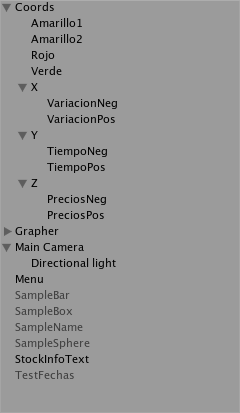
\includegraphics[scale=0.5]{parenting.png}
		\caption{Jerarquía de Objetos en Unity3D.}
	\label{fig:jerarq}
\end{figure}

En este caso, si se rotara/escalára/moviera el objeto `Coords', a su vez a los objetos que se encuentran dentro de `Coords' también se les aplicaría la transformación.\\

Se decidió entonces dividir el programa en 3 grandes módulos principales para facilitar tanto desarrollo como mantenimiento de los contenidos 3D, Dichos modulos le envian información a los otros para renderizar los contenidos 3D. Figura\ref{fig:modules}\\

\begin{figure}[h]
	\centering
		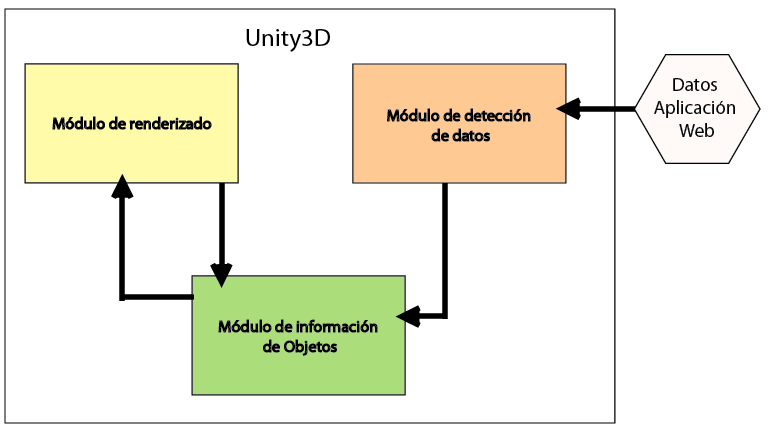
\includegraphics[scale=0.5]{ArquitecturaUnity.png}
		\caption{Arquitectura de los contenidos 3D}
	\label{fig:modules}
\end{figure}


\subsection{Módulo de detección de datos e información del exterior:}
Este módulo se encarga de recibir la información que tiene cada acción que proviene desde la aplicación Web parseándola y organizándola para que los otros módulos de la aplicación la entiendan; posteriormente carga en memoria dicha información para así utilizarla apropiadamente en el tipo de gráfico que se esta renderizando.\\

Este módulo solo es usado cada vez que se le inyectan datos a los contenidos 3D ó cada vez que el usuario pide cambiar el tipo de gráfica a mostrar.\\

\subsection{Modulo de información de Objetos:}
Este módulo se encarga de recolectar la información almacenada en memoria y cargar para cada objeto que se va a mostrar en la escena, la información pertinente del mismo.\\

Este módulo se encarga del manejo de menús y todo lo que tiene que ver con la interacción del usuario con la aplicación, es llamado constantemente cada vez que el usuario desea averiguar información relevante de una acción, y  se comunica una sola vez con el módulo de detección de datos e información del exterior.\\

\subsection{Módulo de renderizado de escena (\emph{Grapher}):}

Finalmente, éste módulo se encarga de lo que es el dibujado de la información proveniente del modulo de información de objetos; éste módulo nunca se entiende con el módulo de datos e información del exterior.\\
 
Para graficar la escena, se recorren todos los nodos que posee el módulo de información y se gráfica (dependiendo del tipo de gráfico) cada nodo.\\


Cabe aclarar que se debe hacer un `vaciado de hijos' del objeto \emph{Grapher} cada vez que se visualizan contenidos, para no introducir \textbf{leaks}\footnote{Ocurre cuando un bloque de memoria reservada no es liberada en un programa de computación. Comúnmente ocurre porque se pierden todas las referencias a esa área de memoria antes de haberse liberado. Dependiendo de la cantidad de memoria perdida y el tiempo que el programa siga en ejecución, este problema puede llevar al agotamiento de la memoria disponible en la máquina.} de memoria.\\



Basicamente 4 tipos de gráficos fueron los que se decidieron desarrollar: Barras, Espiral, Superficie y el Campo. Cada gráfica ofrece información relevante para cada tipo de variable que se esta analizando. \\

\textbf{Barras} [\ref{fig:Barras}:] Son las típicas barras que se pueden encontrar en cualquier visualización de acciones, pero con el valor agregado de que permiten ver el comportamiento de una o varias acciones a través del tiempo.\\

Estas barras muestran variables como el porcentaje de variación, Cantidad negociada, y Precio; Dichos valores son trabajados de modo percentil para poder comparar las otras acciones que tienen precios diferentes, pues una acción puede valer \$5 mientras que otra puede valer \$20000.\\


\begin{figure}[h]
	\centering
		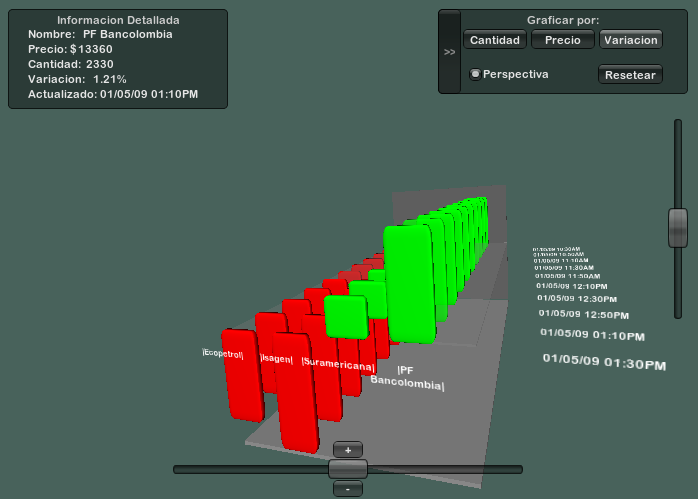
\includegraphics[scale=0.5]{Barras.png}
		\caption{Ejemplo de Visualización por Barras.}
	\label{fig:Barras}
\end{figure}


\textbf{Espiral} [\ref{fig:Espiral}]: Este tipo de gráfica permite comparar rendimientos de varias acciones por medio del porcentaje de variación de cada una en un momento determinado, es el único tipo de gráfico que no permite comparar acciones a través del tiempo, pues lo único que interesa en este gráfico, es determinar de una manera fácil y rápida que acciones están generando mas rentabilidad, cuales están perdiendo y cuales están invariantes en un tiempo dado.\\

\begin{figure}[h]
	\centering
		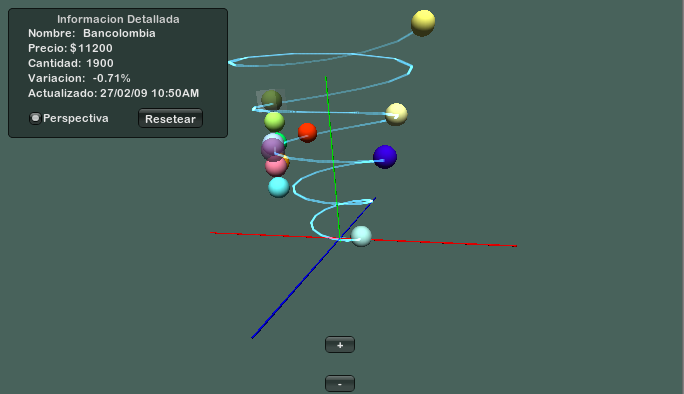
\includegraphics[scale=0.5]{Espiral.png}
		\caption{Ejemplo de Visualización por Espiral.}
	\label{fig:Espiral}
\end{figure}


\textbf{Superficie} [\ref{fig:Superficie}]: Este tipo de gráfico también compara rentabilidades de dos o mas acciones a través del tiempo, con respecto a la mayor/menor rentabilidad de todas las acciones en un momento determinado  mientras que genera una superficie 3D que describe el comportamiento de la bolsa a medida que transcurre el tiempo.\\

\begin{figure}[h]
	\centering
		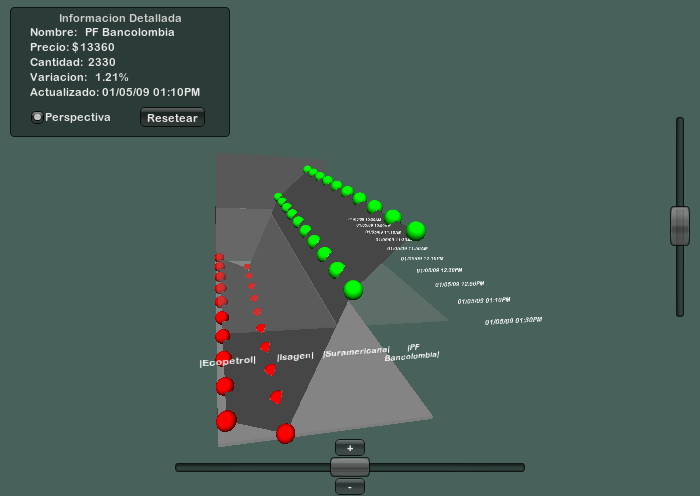
\includegraphics[scale=0.5]{Superficie.png}
		\caption{Ejemplo de Visualización por superficies de rentabilidad.}
	\label{fig:Superficie}
\end{figure}

\textbf{Campo} [\ref{fig:Campo}]: Es el tipo de gráfico mas complejo que se realizó, pues en este gráfico se comparan variables de Cantidad Vs Rentabilidad a través del tiempo, entonces por medio de estas variables se puede inferir si una acción se esta tranzando en la bolsa en mucha cantidad o no y si dicha acción esta siendo rentable; Este gráfico provee una serie de `zonas' que ayudan al usuario a entender el estado de las acciones en un momento dado, y así inferir facilmente si la acción esta generando pérdidas o ganancias y si esta muy o poco demandada\\

\begin{figure}[h]
	\centering
		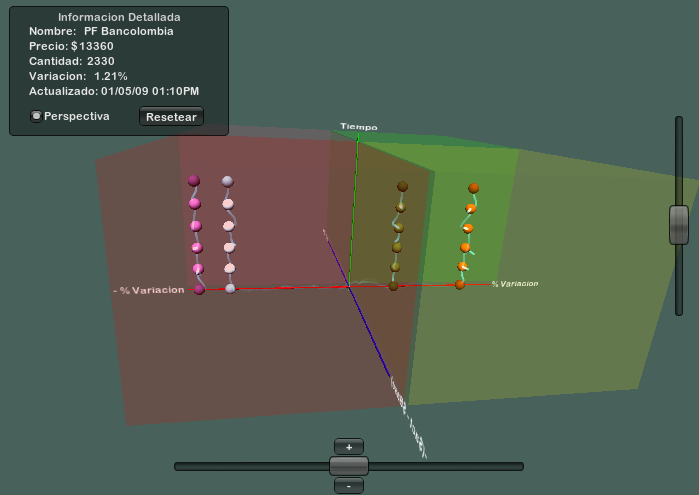
\includegraphics[scale=0.5]{Campo.png}
		\caption{Ejemplo de Visualización por Campos.}
	\label{fig:Campo}
\end{figure}
 

\section{Desarrollo protocolo de comunicación.}

Para el conectar los contenidos 3D con toda la aplicación web, como se mencionó en secciones anteriores, se desarrolló un protocolo escrito en \emph{Javascript}, puesto que \emph{Unity3D} permite el llamado a funciones implementadas dentro del motor por medio de este lenguaje.\\ 

Fue así como por medio de paso de mensajes y llamadas a funciones, se implementó el protocolo de comunicaciones, dicho protocolo actúa como canal sobre el que pasan mensajes a través de funciones nativas de \emph{Javascript} desde la aplicación web (\emph{Ruby} cuenta con una librería especifica para serializar objetos a \emph{Javascript}) a un Objeto \emph{Unity3D} que arroja el \emph{player}, dichas funciónes permiten hacer llamadas nativas a funciones de los contenidos 3D, facilitando este proceso que en un principio pareciera ser más tedioso.\\

El principal problema que se presentó a la hora de diseñar el protocolo fue que el contenido  \emph{HTML} se cargaba antes y mas rápido que el contenido en 3D, lo que conducia eventualmente a la perdida de mensajes y a la incorrecta graficación de los datos. Para solucionar este problema se implementó una llamada desde el contenido 3D a la aplicación web  a través del protocolo que indica cuando un contenido esta listo para recibir datos, y de esta manera graficar correctamente los datos.

A continuación se muestra la parte del protocolo y la función implementada desde el motor, que indica cuando el contenido esta listo para recibir y enviar mensajes.

\begin{verbatim}
write: function (elementId) {
    if(this.detectUnityWebPlayer()) {
        document.write(this.writeEmbedDOM());
        this.findEar();
        return true;
    } else {
        if(this.getAttribute('altHTML') != "") {
            document.write(this.getAttribute('altHTML'));
        } else if(this.getAttribute('redirectUrl') != "") {
            document.location.replace(this.getAttribute('redirectUrl'));
        }
    }
    return false;
},

findEar: function () {
    this.unityEar = "";
    if (navigator.appVersion.indexOf("MSIE") != -1 && 
        navigator.appVersion.toLowerCase().indexOf("win") != -1) {
        this.unityEar = document.getElementById(this.getAttribute('id')+"_object");
    } else if (navigator.appVersion.toLowerCase().indexOf("safari") != -1) {
        this.unityEar = document.getElementById(this.getAttribute('id')+"_object")
    } else {
        this.unityEar = document.getElementById(this.getAttribute('id')+"_embed");
    }
    document.Unity = this.unityEar;
},
   
msg: function (unObj, unFunc, unVar) {
    this.unityEar.SendMessage(unObj, unFunc, unVar);
}
\end{verbatim}

La siguiente porción de código manda una señal hacia el protocolo implementado en \emph{Javascript}, indicando que la aplicación esta lista para renderizar contenidos.\\

\begin{verbatim}
//Funcion implementada en Unity3D
function Update() {
    if(Application.GetStreamProgressForLevel(0) == 1 && !finishedLoadingApp){
        Application.ExternalCall("FinishedLoadingApp");
        finishedLoadingApp = true;
    }
}
\end{verbatim}
\section{\emph{Deployment}}



\section{SCM}
\chapter{Conclusiones}
\begin{itemize}

\item[$\bullet$] Se puede aprovechar las nuevas tecnologías de información, las teorías de ambientes virtuales y las ventajas que ofrece la web 2.0 para potenciar el entendimiento del estado actual de las inversiones. De esta forma se puede observar que las plataformas web pueden ser un gran apoyo para llevar a cabo los procesos de visualización, propiciando entornos que no eran imaginados hace unos años atrás.

\item[$\bullet$] Las gráficas 3D son herramientas de toma de decisiones en el mercado bursátil mas poderosas que las convencionales gráficas bidimensionales, ya que estas ofrecen una visión global del movimiento accionario.

\item[$\bullet$] Las herramientas tecnológicas de visualización + Web2.0 necesitan estar apoyadas en unos lineamientos metodológicos para ayudar a potencializar y agilizar el desarrollo, de otra manera, tener una plataforma que no este testeada o que presente varios problemas, es incurrir en mas esfuerzos y gastos en el proceso de desarrollo

\item[$\bullet$] Aplicar un estándar para el desarrollo de aplicaciones Web 2.0 como el \texttt{TDD} trae grandes ventajas y facilita el manejo y desarrollo de la aplicación, pues de esta forma la misma tendrá unas características mejor desarrolladas en cuanto a reusabilidad, accesibilidad y seguimiento al usuario.

\item[$\bullet$] Antes de desarrollar una aplicación es necesario conocer todo el modelo de negocio de la institución cliente, ya que sin hacer un análisis del entorno es imposible modelar una solución que se adapte a las necesidades específicas y a las características de los usuarios. Del mismo modo, realizar un proceso de planeación previo al desarrollo del producto es importante para distribuir de una forma mejor los recursos disponibles.

\item[$\bullet$] Por medio de la visualización 3D se pueden observar clara y didácticamente los patrones de fluctuación del mercado	

\item[$\bullet$] Utilizar herramientas y plataformas existentes para adaptarlas a las necesidades específicas de la aplicación solicitada trae mucha facilidad, ahorro de tiempo y esfuerzo, pues de esta forma se puede enfocar en las nuevas funcionalidades y en el modelado del problema. En nuestro caso especifico, utilizar y apoyarnos en \emph{Rails} + \emph{Unity3D} para ofrecerle al usuario los servicios requeridos de interacción (Agregar acciones, ganancias diarias, ganancias totales.) fue de gran utilidad porque no fue necesario implementar el sistema desde cero y no se necesitaron crear elementos ya existentes. De esta forma nos pudimos enfocar primordialmente en las necesidades específicas de los jugadores en la bolsa, permitiendo acotar el problema y trayendo finalmente beneficios que se vieron reflejados en el ahorro de tiempo y facilidad de la implementación.	
	
\end{itemize}



\backmatter

\bibliography{tesis}
\bibliographystyle{plain}

\end{document}



